\section{Introduction}
\label{sec:intro}
%Nowadays, advent of consumer friendly and affordable depth-cameras such as Kinect are commercially employed in many applications such as robotics and virtual reality.
%Understanding and interpreting raw data provided by depth-cameras has drawn many attentions of researchers.
%

\comments{
\begin{figure}[t]
	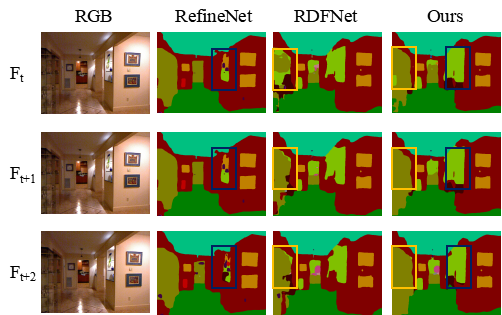
\includegraphics[scale=0.65]{figure/Consist.png}
	\vspace*{-0.6cm} 
	\caption{An illustration of jumping problem in video semantic segmentation. The predicted results of adjacent frames by different methods are shown. Our method generates more temporally consistent results, especially in the highlighted regions.}
	\label{fig:Consist}
	\vspace*{-0.35cm}
\end{figure}
}

Semantic segmentation is a fundamental part of scene understanding.
%
For indoor scenes, the cluttered backgrounds, large variety of scenes, object occlusions and various illumination pose a series of challenges for accurate semantic segmentation.
%
In recent years, a great deal of studies have been conducted for indoor scene semantic segmentation, and they can be mainly divided into three groups: semantic segmentation of a single RGB image, semantic segmentation of RGBD images, and multi-task learning methods.


\noindent \textbf{Semantic Segmentation of a Single Image.}
%
Fully convolutional network (FCN)~\cite{Long2015} is a pioneering work for pixel-wise segmentation. It first converts existing convolutional neural networks (CNN) constructed for classification for semantic segmentation.
%
To overcome the limitations of FCN that the network limited by a fixed-size receptive field, Noh \emph{et al.} \cite{Noh2015} proposed a novel deconvolution algorithm to segment finer object structures.
%
Bayesian SegNet~\cite{Kendall2015} performs visual scene understanding with a measure of model uncertainty to produce a probabilistic segmentation result.
%
To capture semantic correlations between neighboring patches and exploit patch-patch contextual information, Lin \emph{et al.}~\cite{Lin2016} formulated conditional random fields (CRFs) with CNN-based pairwise potential function. 
%
For generating fine prediction, a multi-path refinement network is proposed to effectively exploit multi-level features and refines the prediction step by step~\cite{Lin2017}.
%

\comments{
Semantic segmentation from a single image often leads to incomplete segmentation results. 
%
As the predictions from RefineNet \cite{Lin2017} shown in Fig.~\ref{fig:Consist}.
}

\begin{figure*}[htbp]
%	\vspace{-0.6cm}
	\setlength{\abovecaptionskip}{0pt} 
	\setlength{\belowcaptionskip}{10pt}
	\centering
	\centering
	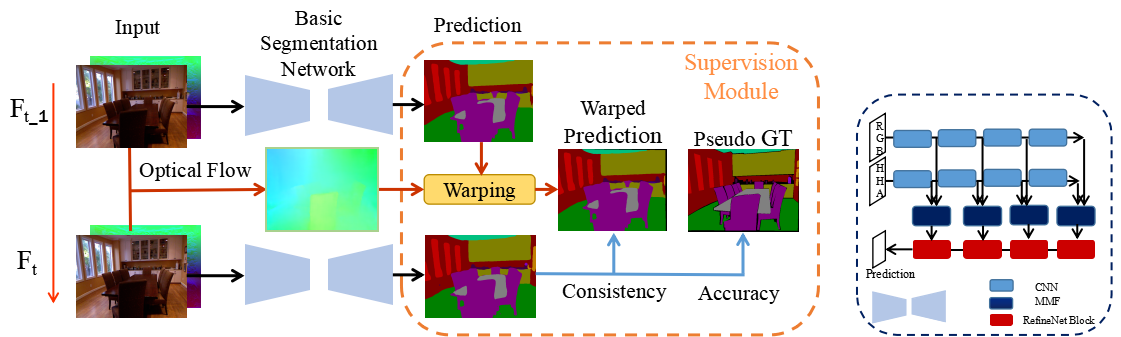
\includegraphics[scale=0.57]{figure/Pipeline.png}
%	\vspace*{-0.8cm} 
	\caption{The diagram of our proposed methods. The left one is pseudo ground truth generation. We propagate the GT from labeled frame to their adjacent frames by image warpping. The right one is flow chart of training segmentation network using temporal consistncy. It mainly consists of three steps: 1) The current frame $F_t$ passes through a basic semantic segmentation network to generate the prediction  2) Warpping the prediction of previous frame $F_{t-1}$ depends on optical flow generated from PWC-Net \cite{Sun2018} 3) Warpped prediction of $F_{t-1}$ and generated PGT joint action on the network by $L_{consistency}$ and $L_{PGT}$ respectively.}
	\label{fig:Pipeline}
	\vspace*{-0.2cm}
\end{figure*}
 

\noindent \textbf{Semantic Segmentation of RGB-Depth Images.}
%
With the popularity of affordable depth-cameras, many techniques have been proposed for semantic segmentation of RGBD images.
%
Gupta \emph{et al.} \cite{Gupta2014} extract features from RGB and depth data and integrate them for object detection and segmentation.
%
A novel long short-term memorized context fusion (LSTM-CF) model is proposed \cite{Li2016} to fuse contextual information from multiple sources such as RGB images and depth data.
% 
Cheng \emph{et al.} \cite{Cheng2017} rethink the relationship between RGB images and depth, and propose a locality-sensitive deconvolution network to refine object boundaries of segmentation result as well as a gated fusion layer to combine features of two modes.
%
Park \emph{et al.} \cite{Park2017} work on fusing the multi-level RGB-D CNN features.
%
They propose a multi-modal feature fusion blocks and added it to RefineNet \cite{Lin2017}.


\textbf{we do not solve the jumping problem.}

{\bf Multi-task Learning.} 
%
Eigen and Fergus \cite{Eigen2015} address three different tasks such as depth prediction, surface normal estimation, and semantic labeling using a single multiscale convolutional netwrok. 
%
Prediction-and-distillationn network (PAD-Net)\cite{Xu2018} predicts a set of intermediate tasks including depth, surface normal, semantic and contour estimation, and then using the predictions from these tasks as multi-modal disitillation modules' inputs for final tasks.  
%
A novel joint Task-Recursive Learning (TRL) \cite{Zhang2018} framework for semantic segmentation and depth estimation was proposed by Zhang \emph{et al}. 
%
In TRL, two tasks are alternately processed in the decoder to imporve each other.
% 
Jiao \emph{et al.} \cite{Jiao2018} presented an attention-driven loss for network supervision and a synergy network to learn the information sharing strategies. 
%
By combining two tasks as well as proposed attention-driven loss, the performance of two tasks are mutuallty improved.
%
Although the multi-task learning methods improve the segmentation results, it needs a lot of supplementary information or even dense-annotated data from other tasks.

Above approaches provide a lot of novel ideas to improve the segmentation results, but the ability and performance of these methods are greatly limited by the limited dense-annotated training data.
%
Meanwhile, dense-annontated data is expensive to obtain.
%
In order to take full use of a large quantity of non-annotated data, in this paper, we propose two simple but effective approaches. 
%
One is propagating labels from annotated frame to neighbouring non-aonnotated frames that generates many good quality and mixed noise pseudo ground truth (PGT) for network training. 
%
Compared to common data augmentation operations, it increases the diversity of training data.
%
The other is proposing a training policy that training a semantic segmentation network with a temporal consistency constraint between frames. 
%
The rest of this paper is organized as follows.
% 
Our methodology will be introduced firstly.
%
Then, we will report the extensive experimental results as well as analyses. 
%
Finally we will draw a conclusion.
